%Exemplo de capitulo

\chapter{Implementação e Experimentos}

Neste capítulo será apresentada uma implementação do método descrito
no capítulo \ref{ses:metodo}. Esta implementação será usada para medir o
desempenho do método proposto segundo métricas padronizadas, além de métricas
adicionais.

Também será apresentado um breve histórico mostrando algumas abordagens que
foram tentadas antes da implementação final ter sido obtida, mostrando por que
elas falharam.

\section{Arquitetura Global}
Redes neurais em geral requerem grande quantidade de exemplos de treinamento
para evitar \emph{overfitting} \cite{hawkins2004problem}. É crucial para o
sucesso de uma implementação acesso a dados ou a capacidade de produzi-los.

\begin{figure}[!htb]
	\centering
	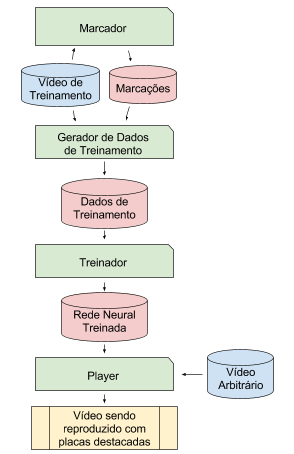
\includegraphics[scale=1]{cap5_arquit_global.png}
	\caption{Arquitetura Global da Implementação}
	\label{fig:cap5_arquit_global}
	Diagrama ilustrando os quatro componentes de \emph{software} em verde, os
	vídeos
	de entrada em azul, as informações intermediárias em vermelho e a saída do
	sistema em amarelo (próprio autor).
\end{figure}

Durante a faze conceitual optou-se por dar um grande enfoque no
treinamento da rede neural. Como não existe nenhuma fonte pública de imagens
etiquetadas de placas de carro com as características necessárias optou-se por
gerar estes dados a partir de imagens de vídeo.
Para tal, dois módulos foram desenvolvidos: um de
marcação manual de placas em vídeo e um para geração desses dados.
Usando os dois é possível gerar exemplos rotulados em quantidade
suficiente no formato requerido pela rede neural. O treinamento e os testes
requereram o desenvolvimento de outros dois outros módulos: o primeiro
treina a rede neural, o segundo reproduz o vídeo enquanto aplica a rede neural
treinada, mostrando as placas identificadas. Isso resulta em quatro módulos de
\emph{software} principais. O relacionamento entre eles é mostrado na figura
\ref{fig:cap5_arquit_global}.

A implementação de cada um destes módulos mudou durante a história do projeto,
porém as suas funções básicas permaneceram as mesmas.

\section{Abordagens Anteriores}
Durante o desenvolvimento do projeto algumas tentativas mal sucedidas foram
feitas antes da versão final ter sido completada. O \emph{software} chegou a
ser implementado por completo três vezes, sendo que só produziu resultados
satisfatórios na última.

A ideia inicial para este projeto era o uso de redes neurais não-convolucionais
aplicadas diretamente aos \emph{pixels} das imagens. Para tal foi escolhida a
biblioteca \emph{neuroph}, devido à familiaridade e ao uso da linguagem Java. A
solução foi totalmente implementada conforme arquitetura ilustrada na figura
\ref{fig:cap5_arquit_global}.

Essa implementação usava imagens em tons de cinza e partições com dimensões HW
$32 \times 100$ aplicadas em uma rede neural totalmente conectada com 3200
entradas e uma saída. O particionamento era feito usando \emph{stride} de
100\%, ou seja, duas partições vizinhas tinham o perímetro de um dos seus
lados em comum.

Esta biblioteca foi logo descartada porque o tempo de treinamento era muito
longo, impedindo a busca eficiente de configuração das camadas ocultas que
gerasse o resultado desejado. Testes com topologias mais complexas, com maior
largura e profundidade nas camadas intermediárias, chegavam a passar de uma
semana de execução quando rodadas em um notebook \emph{Core i7}. Não houve
nenhuma configuração encontrada com desempenho de classificação aceitável.

Acreditando que seria possível resolver o problema encontrando os
hiperparâmetros corretos da rede neural, e sabendo que isso requeriria
múltiplos experimentos com topologias diferentes, adotou-se a biblioteca
\emph{encog},
devido ao melhor desempenho de treinamento. Essa adaptação, requereu reescrever
boa parte código. Apesar do treinamento rodar a uma taxa de imagens 10
vezes maior que a biblioteca anterior, também não foi encontrada topologia
com desempenho aceitável. A figura
\ref{fig:cap5_trein_redes_nao_conv} mostra a
evolução do treinamento para algumas sessões. Entre as listadas a que teve
melhor desempenho usava 3200 neurônios na camada de entrada, então 172, 137,
109, 87, 69, 55, 44, 35 e 28 neurônios nas camadas ocultas, terminando
com uma saída.

\begin{figure}[!htb]
	\centering
	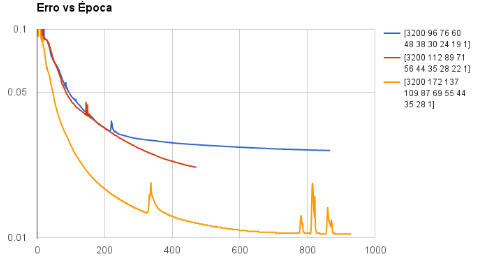
\includegraphics[scale=0.75]{cap5_trein_redes_nao_conv.png}
	\caption{Erro de treinamento de redes neurais não-convolucionais}
	\label{fig:cap5_trein_redes_nao_conv}
	A ordenada refere-se ao erro L2 calculado sem a raiz quadrada e suavizado
	usando \emph{exponential smoothing}. A legenda refere-se ao número de
	neurônios em cada camada totalmente conectada (próprio autor).
\end{figure}

Quando o \emph{player} era usado com as redes neurais resultantes
desse treinamento o
resultado era muito ruim, com quantidade muito grande de falsos negativos.
Eventualmente descobriu-se que a forma com que os exemplos de imagens que não
continham placa estava sendo coletada possuía uma grande quantidade de imagens
muito parecidas. Aparentemente a rede neural não estava conseguindo generalizar
as características de uma placa veicular e, ao invés disso, encontrou
parâmetros para as camadas totalmente conectadas que identificavam corretamente
alguns destes exemplos, o que acabava reduzindo o erro de treinamento até certo
ponto. A redução das imagens parecidas no set de treinamento de entrada só
foi feito depois das redes neurais totalmente conectadas terem sido
abandonadas.

O esquema de particionamento das imagens foi mudado de 100\% para 50\%, que é o
valor usado agora. A função que a rede neural modela foi modificada
várias vezes, mas o resultado final, conforme visto no \emph{player},
continuava ruim.

Após alguns meses a abordagem foi abandonada. Foi feita uma pesquisa sobre o
assunto descobriu-se a existência de redes neurais convolucionais. Infelizmente
a biblioteca \emph{encog} e a \emph{neuroph} não suportam este tipo de
topologia. Também não foram encontradas bibliotecas com grande base de
usuários em Java.

Neste ponto foi escolhida a biblioteca recém-lançada \emph{TensorFlow}.
Inicialmente a
preparação dos dados de treinamento continuou sendo feita pelo código em Java
que já havia sido escrito, enquanto o código de treinamento e execução foram
reescritos em Python, que era a única linguagem suportada quando essa
migração foi realizada.

O uso de duas linguagens de programação estava eliminando várias oportunidades
de reuso de código. Eventualmente os \emph{softwares} de marcação e preparação
de dados de treinamento foi reescrito em Python.

Desde os primeiros experimentos a abordagem usando redes neurais foi muito bem
sucedida. A primeira abordagem foi usando regressão logística. No entanto os
exemplos de treinamento foram etiquetados de usando apenas valores 0 e 1. Por
não saber exatamente como mapear uma placa parcialmente visível para
probabilidades, foi feita a migração para um modelo de regressão, onde uma
função suave pode ser definida para ser imitada pela rede neural.

\section{Escolha de Tecnologias}
A versão final da DCNN usa o \emph{framework} \emph{TensorFlow} do Google.
No \emph{TensorFlow} usa-se a linguagem Python para descrever um ou mais
grafos onde
os nós são operações e as arestas são tensores. Uma vez que o grafo esteja
totalmente definido podem-se fornecer dados e solicitar o cálculo de qualquer
quantidade de nós. A execução em si ocorre em um \emph{runtime} de alto
desempenho escrito em C++ e CUDA, que pode ser distribuído entre múltiplas
máquinas e pode rodar em CPUs e GPUs.

A tecnologia foi escolhida por ser \emph{open source}, e por ser a ferramenta
utilizada pelo Google. Esta biblioteca é fácil de usar para pequenos projetos,
como este, e poderosa para poder escalar para sistemas com múltiplos
computadores usando GPUs de alto desempenho. O \emph{TensorFlow} permite usar
Python 2 ou Python 3, sendo que a versão 3 foi escolhida para o projeto.

A versão 3 do OpenCV, bem como seu \emph{wrapper} Python foram adotados para
leitura e exibição do vídeo, e para algumas operações de manipulação de
imagens e para a construção da interface com usuário. O OpenCV tem
funcionalidades suficientes para exibir uma janela contendo
uma imagem e capturar eventos de teclado e mouse. Isso é suficiente para toda a
interface gráfica.

Tanto o \emph{wrapper} Python do OpenCV quanto o \emph{TensorFlow} representam
dados numéricos, como tensores, usando uma biblioteca numérica para
Python chamada \emph{numpy}. Ela foi usada para várias operações, como
extrair sub imagens
das \emph{frame} de vídeo, após terem sido lidas pelo OpenCV, e fornecer
estes dados para o \emph{TensorFlow}.

Para representar as marcações que o usuário faz nos vídeos, para identificar
onde estão as placas, foi usado o formato \sigla{JSON}{\emph{JavaScript
object notation}, notação de objetos do \emph{JavaScript}}.
Existem boas
bibliotecas em várias linguagens, inclusive Python e Java, o que garante que os
dados poderão ser lidos facilmente.

O Linux foi o único sistema operacional usado, por ser \emph{open source},
gratuitamente acessível e poder ser usado em produtos comerciais, caso surja a
demanda. A distribuição escolhida foi Arch Linux, apesar de não ser
oficialmente suportado pelo projeto \emph{TensorFlow}, por possuir a filosofia
empregar sempre a versão mais atual de todos os componentes, como kernel. O
suporte ao \emph{TensorFlow} é oferecido pela comunidade
\sigla{AUR}{\emph{Arch User
Repository}} (Arch User Repository), que permite a instalação a partir do
código-fonte do \emph{TensorFlow} mesmo antes de uma versão oficial ser liberada.

O sistema de controle de versões usado foi o GIT.
Esse \sigla{VCS}{\emph{Version control system}, sistema de controle de versão}
já é usado no projeto \emph{TensorFlow}.

Para edição de código foi usado exclusivamente vim. Esse editor é sofisticado
e produtivo quando usado com uma linguagem como Python.

\section{Recursos de Hardware}

O único recurso de hardware que foi necessário para este projeto foi
um computador, sendo que dois foram usados:

\begin{itemize}
\item Um notebook Core i7-3632QM com 4 cores (2 threads por core), 16 GiB
	de RAM;
\item Um notebook Core i5-4210U com 2 cores (2 threads por core), 8 GiB de RAM,
	placa de video NVidia GT-750M com 2 GiB de RAM compatível com
	\emph{TensorFlow}.
\end{itemize}

O desenvolvimento do projeto foi quase todo feito usando o Core i7. Assim que
o suporte a GPU foi incluída no código o notebook Core i5 começou a ser usado
concomitantemente.

A \sigla{CPU}{\emph{Central processing unit}, central unificada de
processamento} do computador Core i7, quando usado para treinamento, rapidamente
atinge \SI{85}{\degree} e o desempenho do treinamento reduz consideravelmente,
como consequência da CPU estar atuando para limitar a potência dissipada. Após
o computador rodar por alguns meses desta maneira o computador deixou de ser
confiável, travando com frequência e muitas vezes se recusando a ligar com
sintomas aleatórios. No caso de treinamento prolongado, como foi feito neste
projeto, pode ser necessário conferir a temperatura na qual os componentes
estão rodando, para evitar danos.

\section{Implementação dos Módulos de \emph{Software}}

Nesta seção está detalhada a implementação de cada módulo de \emph{software}.

\subsection{Marcador}

\begin{figure}[!htb]
	\centering
	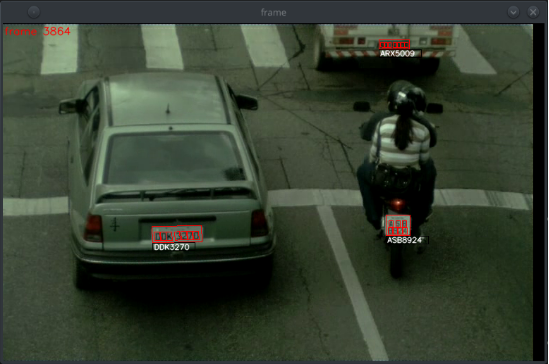
\includegraphics[scale=0.75]{cap5_tela_marcador.png}
	\caption{Interface com usuário do \emph{Marcador}}
	\label{fig:cap5_tela_marcador}
	A tela está mostrando 3 veículos marcados (próprio autor).
\end{figure}

O \emph{software} marcador foi construído como um script Python que recebe o
nome de um arquivo de vídeo como parâmetro. Ele permite:

\begin{enumerate}
\item Reproduzir o vídeo;
\item Pausar a reprodução do vídeo
\item Avançar / voltar frame-a-frame;
\item Saltar para uma \emph{frame} digitando-se o número dela;
\item Quando o vídeo está em pausa, permite clicar no vídeo para adicionar um
	marcador de placa;
\item Usar o teclado para mover, rotacionar e alterar o marcador, de forma que ele
	circule corretamente a placa sendo marcada;
\item Digitar o número da placa veicular
\end{enumerate}

Como pode ser visto na figura \ref{fig:cap5_tela_marcador}, o \emph{software}
marcador permite marcar placas de
carros e motos, e é possível identificar o número da placa. Isto tem como
objetivo permitir que as mesmas marcações possam ser usadas futuramente para
fazer OCR das placas. As marcações são salvas em um arquivo JSON.

Quando uma \emph{frame} possui pelo menos uma placa veicular marcada, todo
o resto da
imagem vai ser considerado pelo \emph{software} de treinamento como região
sem placa.  Por isso, se uma placa for marcada em uma \emph{frame}, devem-se
marcar todas as placas.

\begin{table}
	\center
	\caption{Arquivos de vídeo usados durante o desenvolvimento}
	\renewcommand{\arraystretch}{1.6}
	\begin{tabular}{ccccc}
		\Xhline{6\arrayrulewidth}
		\textbf{Vídeo} &
			\textbf{Resolução} &
			\textbf{FPS} &
			\textbf{Tamanho} &
			\textbf{Duração} \\
		\Xhline{2\arrayrulewidth}
		video1.avi & $480 \times 768$   & 25,0 & 141 MiB & 8:27  \\
		video2.avi & $1080 \times 1920$ & 25,0 & 1,0 GiB & 36:16 \\
		video3.avi & $1080 \times 1920$ & 25,0 & 465 MiB & 8:02  \\
		\Xhline{6\arrayrulewidth}
	\end{tabular}
	\label{tbl:videos}
\end{table}

Todo o desenvolvimento foi feito usando três vídeos. As características dos
vídeos estão listadas na tabela \ref{tbl:videos}, e uma \emph{frame} de
cada vídeo está mostrada na figura \ref{fig:cap5_3_videos}.

\begin{figure}[!htb]
	\centering
	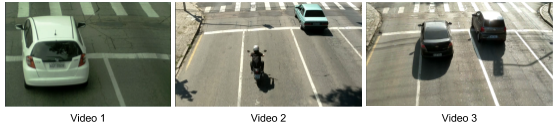
\includegraphics{cap5_3_videos.png}
	\caption{Uma \emph{frame} de cada vídeo usado durante o desenvolvimento}
	\label{fig:cap5_3_videos}
	(próprio autor).
\end{figure}

A tabela \ref{tbl:marc_videos} mostra a quantidade de marcações feitas em cada
vídeo. A maior parte das marcações foram feitas no \emph{video1}. Observar que
existe dois sets de marcações neste vídeo. Uma delas, denominada
\emph{testes}, não foi usada para treinamento, pois está reservada para
testar o desempenho do modelo. Os dados de treinamento estão todos antes do
\emph{frame} número 8000, e todos os dados de teste vêm depois.

\begin{table}
	\center
	\caption{Marcações feitas em cada vídeo}
	\renewcommand{\arraystretch}{1.6}
	\begin{tabular}{c c c}
		\Xhline{6\arrayrulewidth}
		\textbf{Vídeo} &
			\textbf{Quadros Marcados} &
			\textbf{Placas Marcadas} \\
		\Xhline{2\arrayrulewidth}
		video1.avi & 191 & 233 \\
		video1.avi (testes) & 90 & 92 \\
		video2.avi & 71  & 96  \\
		video3.avi & 0   & 0   \\
		\Xhline{6\arrayrulewidth}
		TOTAL      & 352 & 421 \\
	\end{tabular}
	\label{tbl:marc_videos}
\end{table}

\subsection{Gerador de Dados de Treinamento}

\begin{figure}[!htb]
	\centering
	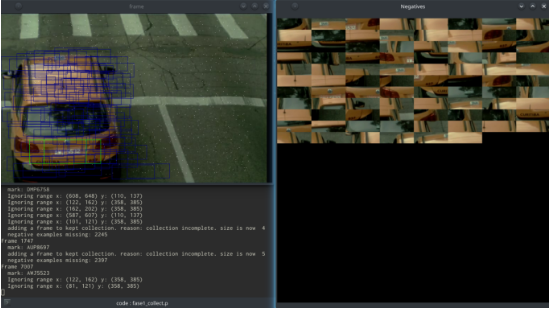
\includegraphics{cap5_tela_gerador.png}
	\caption{Interface gráfica do gerador de dados}
	\label{fig:cap5_tela_gerador}
	A imagem da esquerda mostra o quadro que está sendo processado e mostra as
	regiões onde os exemplos negativos estão sendo coletados. A imagem da
	direita mostra os próprios exemplos negativos que estão sendo enviados para
	o arquivo (próprio autor).
\end{figure}

O \emph{software} gerador de dados de treinamento também recebe como parâmetro
o nome do arquivo de vídeo onde vai operar, e vai abrir este arquivo de vídeo
e as marcações feitas nele. Este \emph{software} roda de modo não-interativo,
terminando sem intervenção do usuário quando a geração do conjunto de
treinamento está concluída. A interface gráfica está ilustrada na figura
\ref{fig:cap5_tela_gerador}

O conjunto de treinamento é armazenado em formato binário contendo registros de
tamanho fixo. Cada registro contém a imagem seguida de um rótulo. A
imagem é codificada no formato HWC usando 1 byte por canal de cor,
sendo a cor na ordem RGB. O rótulo representa o valor que a rede neural
deve aprender (número ponto-flutuange de 0 à 1), mas é codificado como um
inteiro de
8 bits sem sinal.  Como a imagem é $40 \times 120 \times 3$ e o rótulo
tem 1 byte, então cada registro possui 14401 bytes.

Este \emph{software} lê a lista de \emph{frames} marcadas em uma ordem
aleatória. Então vai coletar exemplos de placas veiculares centradas e fora
de centro e exemplos de imagens que não contém placas, e vai salvá-las no
arquivo de saída. A cada um dos exemplos de treinamento este \emph{software}
também salva um número que é o valor da função que a rede neural deve
produzir para esta placa, conforme equação \ref{eq:funcao_a_modelar}.

Tomando uma placa nas coordenadas $y \times x$, o \emph{software} primeiro gera
um recorte centrado nessas coordenadas e com o tamanho $40 \times 120$. Este
tamanho é definido em um arquivo de configuração. Todos os exemplos
coletados desta forma recebem o rótulo 1 (codificado como 255).

Para obter os exemplos de placas não centralizadas são coletados recortes
com dimensões $40 \times 120$ de
aproximadamente 4 em 4 \emph{pixels} dentro de uma região próxima da placa. O
algoritmo avança precisamente na taxa de 4 \emph{pixels}, porém adiciona um
número aleatório de -2 à 2 em cada um deles. Isso tem como objetivo evitar de
fornecer dados muito regulares para a rede neural para evitar que ela
aprenda algum truque relacionado à este padrão de distância. A região onde
coleta-se estes exemplos é tal que o centro fica dentro de uma região
$40 \times 120$ centrada na placa do veículo, como ilustrado na figura
\ref{fig:cap5_regiao_coleta_amostras}.

\begin{figure}[!htb]
	\centering
	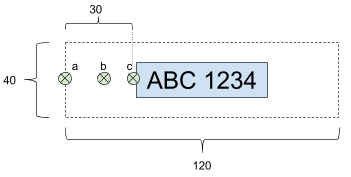
\includegraphics{cap5_regiao_coleta_amostras.png}
	\caption{Região onde amostras são coletadas}
	\label{fig:cap5_regiao_coleta_amostras}
	Esta região delimita os centros das partições, então \emph{pixels} fora
	dessa região são coletados. Partições centrados dentro da região delimitada
	são coletados de 4 em 4 \emph{pixels}, sendo que cada uma dessas regiões é
	deslocada 2 \emph{pixels} para a direita ou para a esquerda. Em verde estão
	marcados três pontos, a, b e c, que serão atribuídos respectivamente aos
	rótulos 0, $^1/_2$ e 1 (próprio autor).
\end{figure}

A região delimitada é exatamente a região na qual o valor é não-zero. O ponto
(c) na figura \ref{fig:cap5_regiao_coleta_amostras} mostra o limiar que está
a $^1/_4$ de distância do centro na direção da largura. Neste ponto a função
começa a decair de 1 para 0 (que são codificados como 255 e 0). O ponto (a)
é onde a função atinge o valor 0, e o ponto (b) está precisamente no
meio do caminho, possuindo o valor 0,5 (codificado como 128).

Após coletar os exemplos de placas contidas na região acima indicada ocorre a
coleta de imagens fora da região, denominada coleta de “exemplos negativos”. A
todos os exemplos coletados dessa maneira é atribuído o rótulo 0.

O algorítmo que coleta esses exemplos passou por vários aprimoramentos. A
versão final, que vai ser descrita, melhorou consideravelmente o desempenho do
treinamento comparado com as versões iniciais.

A primeira, e mais importante otimização foi a eliminação de exemplos
parecidos. Quando são coletados exemplos de regiões da imagem que não são
placas de carro pode-se acabar obtendo um recorte que inclui apenas o asfalto.
Se outro recorte for feito em outra \emph{frame} na mesma região pode acabar
sendo um exemplo muito parecido, como ilustrado na figura
\ref{fig:cap5_coleta_negativa_igual}.

\begin{figure}[!htb]
	\centering
	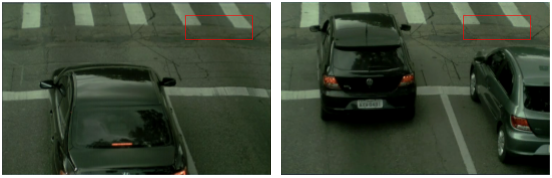
\includegraphics{cap5_coleta_negativa_igual.png}
	\caption{Exemplo de duas regiões iguais em frames diferentes}
	\label{fig:cap5_coleta_negativa_igual}
	As regiões possuem as mesmas coordenadas, e contém \emph{pixels} de fundo
	da imagem (próprio autor).
\end{figure}

Por este motivo o \emph{software} mantém as últimas 100 \emph{frames} processadas.
Quando um “exemplo negativo” vai ser coletado em uma região a imagem é
comparada com os \emph{pixels} da mesma região nestas \emph{frames} que foram
armazenadas. O critério de comparação é:

\begin{equation}
	d_C=\frac{1}{N} \sum_{n=1}^N \sqrt{\left| R_C [n] -I_C [n] \right|}
\end{equation}

Onde $R_C[n]$ é o valor do canal de cor “C” do n-ésimo píxel da partição de
referência, e $I_C[n]$ é o mesmo canal do n-ésimo \emph{pixel} da
partição que está sendo testada. Quando o valor da média dessa métrica
para os três canais é menor que $\sqrt{8}$ as imagens são consideradas
semelhantes, e a amostra é recusada. Foram
testadas métricas, como média do módulo da diferença, e média da diferença
quadrática, mas tiveram desempenho inferior ao serem comparados usando a
percepção humana como referência. A figura
\ref{fig:cap5_tela_gerador} mostra o efeito desta otimização.
Cada retângulo azul mostra a região onde um exemplo negativo foi coletado.
Observa-se que o asfalto não está sendo coletado.

A segunda otimização foi a distância entre duas amostras negativas. Duas
amostras muito próximas tem pouco valor para treinamento da rede neural devido
à invariância a deslocamento. Por isso, para uma amostra ser aceita como
“exemplo negativo” ela precisa estar a mais de 4 \emph{pixels} de todos os
outros exemplos coletados.

A terceira otimização foi o processo de escolha das coordenadas onde os
exemplos são coletados. Inicialmente usava-se um grid regular, mas essa
abordagem acabava coletando uma quantidade muito grande de exemplos negativos.

Como isso a rede neural acabava aprendendo a favorecer valores negativos, pois
errar “para mais” acabava sendo punido mais severamente que errar “para menos”
durante a otimização. Para poder balancear a quantidade de exemplos negativos e
positivos foi necessário substituir o grid linear, já que ele favorecia coletar
exemplos negativos na parte superior da imagem, pois a coleta terminava antes
da imagem chegar na parte inferior.

Para resolver isso foi adotado um processo que escolhe coordenadas usando uma
distribuição uniforme e testa se nas coordenadas existe um exemplo negativo
válido. Infelizmente este algoritmo é $O(\infty)$ no pior caso. Por isso um
novo algoritmo de busca
que tem probabilidade próxima de uniforme para a busca, vai sempre encontrar
todas as soluções, e sempre termina precisou ser criado. Este algoritmo é uma
modificação do BFS (\emph{breadth-first search}), no no qual a ordem na
qual a busca é adicionada à pilha é aleatória. O algoritmo pega
de uma pilha uma região
retangular na qual deve encontrar pontos válidos e usa um gerador aleatório
uniforme para escolher coordenadas e testar. Se o teste falhar divide a região
em duas sub-regiões na direção onde a imagem for maior (altura ou largura) e
adiciona as regiões na pilha em ordem aleatória. Cada vez que coordenadas
válidas são encontradas elas são adicionadas na lista de resposta. Se a lista
possui o número solicitado de respostas o algoritmo termina, caso contrário
continua.

\begin{table}
	\center
	\caption{Exemplos de treinamento gerados para cada vídeo}
	\renewcommand{\arraystretch}{1.6}
	\begin{tabular}{c c c p{2.5cm} p{2.5cm}}
		\Xhline{6\arrayrulewidth}
		\textbf{Entrada} &
			\textbf{Saída} &
			\textbf{Tamanho} &
			\textbf{Registros \newline Gerados} \\
		\Xhline{2\arrayrulewidth}
		video1.avi & video1.nn1.bin & 1,1 GiB  & 64.714  \\
		video2.avi & video2.nn1.bin & 901 MiB  & 89.672  \\
		\Xhline{6\arrayrulewidth}
		TOTAL      &                & 2,07 GiB & 154.386 \\
	\end{tabular}
	\label{tbl:ex_marc_videos}
\end{table}

Um script escrito em bash foi escrito partir um arquivo destes em arquivos
menores, contendo 128 amostras cada. Isso gerou 630 arquivos a partir de
\emph{video1.nn1.bin} e 240 arquivos a partir de \emph{video2.nn1.bin}.

Finalmente, um diretório foi criado contendo links simbólicos para todos os 869
arquivos. Este diretório é o resultado final da geração de exemplos, e contém
todas as amostras coletadas de todos os vídeos.

\subsection{Treinador}

\begin{figure}[!htb]
	\centering
	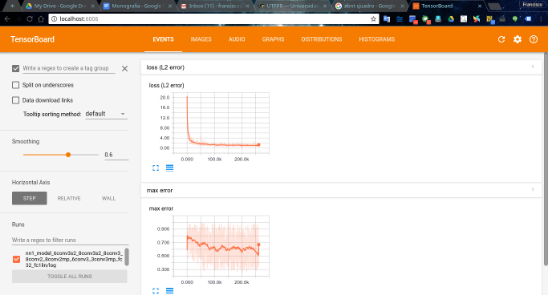
\includegraphics{cap5_tela_treinador.png}
	\caption{Página do \emph{TensorBoard} mostrando progresso do treinamento}
	\label{fig:cap5_tela_treinador}
	Esta é uma página \emph{web} que permite observar a evolução do
	treinamento (próprio autor).
\end{figure}

O treinador é um módulo de \emph{software} onde se configura uma topologia de rede
neural convolucional, que é treinada usando os dados produzidos pelo gerador de
dados de treinamento.

Para realizar o treinamento tanto da rede neural um grafo apresentado na figura
\ref{fig:cap5_grafo_treinamento} foi construído.

\begin{figure}[!htb]
	\centering
	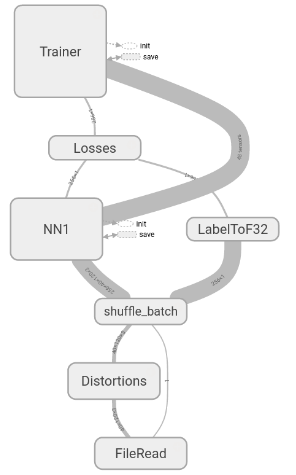
\includegraphics[scale=0.7]{cap5_grafo_treinamento.png}
	\caption{Grafo usado para treinamento da rede neural convolucional}
	\label{fig:cap5_grafo_treinamento}
	Esta imagem mostra o grafo do \emph{TensorFlow} usado para treinar
	a rede neural, que é o bloco \emph{NN1} (próprio autor).
\end{figure}

O bloco “FileRead” possui uma lista com todos os arquivos de treinamento
gerados pelo gerador de exemplos de treinamento. Essa lista é embaralhada, e
então cada um dos registros é lido em sequência. A imagem é representada por um
tensor de inteiros de 8 bits com dimensões $40 \times 120 \times 3$, e o
rótulo da imagem é representado com um tensor unidimensional com dimensão $1$.

Como a rede neural está sendo treinada usando apenas dois vídeos existe o risco
da rede neural treinada fique muito sensível a fatores como a iluminação. Para
impedir que isso aconteça as imagens são distorcidas durante o treinamento no
bloco de distorções, que está ilustrado na figura \ref{fig:cap5_distorcao}.
A imagem é convertida para ponto-flutuante com canais no intervalo $[0;1]$,
conforme requerido pelos primitivos do próprio \emph{TensorFlow}.
No final das distorções a imagem é convertida
novamente para inteiro de 8 bits por canal. O motivo para isso é fazer com o
que o bloco “NN1”, que implementa a rede neural seja o mais otimizado possível
para classificar imagens, não tanto para treinamento.

\begin{figure}[!htb]
	\centering
	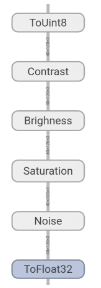
\includegraphics{cap5_distorcao.png}
	\caption{\emph{Pipeline} de distorção de imagens}
	\label{fig:cap5_distorcao}
	A imagem é convertida para ponto-flutuante com cada canal no intervalo
	$[0;1]$, é adicionado ruído normal, a saturação, brilho e contraste são
	alterados conforme uma distribuição normal. O número é então convertido
	novamente para inteiro de 8 bits por canal (próprio autor).
\end{figure}

O bloco “Noise” adiciona ruído normal à imagem somando-a com um tensor com as
mesmas dimensões onde o valor de cada canal é gerado por uma distribuição
normal de média 0 e desvio padrão 0,06.

O bloco “Saturation” altera a saturação entre 0,2 a 1,5, sendo que 1 representa
manter a saturação inalterada. O bloco “Brightness” faz uma alteração no brilho
aumentando ou diminuindo em até 40\%. O bloco “Contrast” faz uma alteração de
contraste entre 0,6 e 1,4, sendo que 1 representa manter o brilho. As escolha
do valor em todos os casos é aleatória de acordo com distribuição uniforme.

O resultado das distorções, juntamente com o rótulo da imagem são fornecidos
para o bloco “shuffle\_batch”. Este bloco tem a função de embaralhar os
dados e agrupar imagens em batches. Este bloco usa 8 threads para consumir
os dados dos blocos anteriores, o que significa que leitura e shuffling vai
ocorrer em paralelo. Quando 2560 imagens são lidas elas são embaralhadas
elas são agrupadas em batches de 256 imagens, gerando tensores com
dimensões $256 \times 40 \times 120 \times 3$. Como cada arquivo contém
128 registros, então as imagens
sendo lidas contém, no pior caso, uma amostra aleatória proveniente de 20
arquivos. Os arquivos em sí são lidos em ordem aleatória, o que gera uma
amostragem razoavelmente diversa das informações de entrada.

Quanto maior o tamanho do batch maior a precisão da estimativa de erro,
portanto este número é o maior possível suportado pelo hardware onde o
treinamento está sendo realizado.

Se o treinamento for rodado por tempo suficiente, todas as imagens serão
lidas. Se o treinador precisar de mais exemplos as mesmas imagens serão lidas
novamente, em ordem diferente. Porém, graças ao sistema de distorção de
imagens que é parte do pipeline de leitura, uma mesma imagem lida múltiplas
vezes muito provavelmente não chegará idêntica na rede neural.

Os tensores que saem do shuffler são fornecidos a rede neural, que está no
bloco “NN1”, que está ilustrado na figura \ref{fig:cap5_cnn}.

\begin{figure}[!htb]
	\centering
	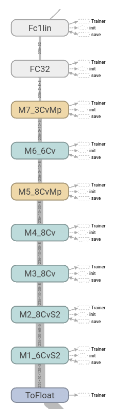
\includegraphics{cap5_cnn.png}
	\caption{Pipeline descrevendo a rede neural convolucionao profunda}
	\label{fig:cap5_cnn}
	(próprio autor)
\end{figure}

Pode-se ver pela espessura das linhas que conectam os blocos que a quantidade
de informação reduz ligeiramente em cada etapa. Como a rede neural precisa
de um tempo de propagação baixo algumas técnicas foram usadas para
reduzir o número de computações.

A primeira estratégia é a redução agressiva do tamanho dos tensores nas duas
primeiras camadas, inspirado em \cite{szegedy2015going}. \emph{Stride} é usado
para fazer um resampling da imagem. Este método usa mais CPU do que resampling
por métodos como bilinear, porém permite acesso à textura da imagem original. A
primeira camada usa um kernel de $2 \times 2$ ao invéz de $3 \times 3$,
reduzindo o número de multiplicações de 9 para 4.

Não está sendo usada nenhuma convolução maior que $3 \times 3$.
\cite{szegedy2015going} defende que, pelo menos em alguns casos,
convoluções $5 \times 5$ podem ser substituídas por duas convolução
sucessivas $3 \times 3$ enquanto reduz o número de
multiplicações de $25$ para $2 \cdot 9=18$.

\begin{table}
	\center
	\caption{Camadas da Rede Neural Implementada}
	\renewcommand{\arraystretch}{1.6}
	\begin{tabular}{c c c c}
		\Xhline{6\arrayrulewidth}
		\textbf{Nome} &
			\textbf{Tensor de Entrada} &
			\textbf{Operação} &
			\textbf{DOF} \\
		\Xhline{2\arrayrulewidth}
		M1 & $256 \times 40 \times 120 \times 3$ & 6 cv2x2 s2x2 relu  & 78   \\
		M2 & $256 \times 20 \times 60 \times 6$  & 8 cv3x3 s2x2 relu  & 440  \\
		M3 & $256 \times 10 \times 30 \times 8$  & 8 cv3x3 relu       & 584  \\
		M4 & $256 \times 10 \times 30 \times 8$  & 8 cv3x3 relu       & 584  \\
		M5 & $256 \times 10 \times 30 \times 8$  & 8 cv3x3 relu mp2x2 & 584  \\
		M6 & $256 \times 5  \times 15 \times 8$  & 6 cv3x3 relu       & 438  \\
		M7 & $256 \times 5  \times 15 \times 6$  & 3 cv3x3 relu mp2x2 & 165  \\
		-  & $256 \times 3  \times 8 \times 3$   & flatten            & 0    \\
		FC32 & $256 \times 72$                   & fc32 relu          & 2.336\\
		FC1 & $256 \times 32$                    & fc1 linear         & 33   \\
		SAÍDA & $256$                            &                    &      \\
		\Xhline{6\arrayrulewidth}
		TOTAL & & & 5.242 \\
	\end{tabular}
	\label{tbl:camadas_cnn}
\end{table}

Nas últimas camadas está sendo usado maxpool $2 \times 2$. Esta estratégia é
computacionalmente mais cara que usar convolução com stride maior que 1, pois
de cada 4 valores 3 deles são descartados. Como as imagens são menores no final
da rede neural optou-se pela operação mais cara. O efeito em tempo de
propagação é negligenciável, o efeito na qualidade da detecção não foi medido.

Outro ponto importante é o controle do número de graus de liberdade. Os
primeiros modelos tinham mais de 50.000 graus de liberdade, e este valor foi
reduzido para 5.242. Menos parâmetros implica várias vantagens, como
treinamento mais rápido, menos uso de memória, capacidade de usar
\emph{batches} maiores e menor chance de \emph{overfitting}.

O processo que mais ajudou a aprimorar sucessivamente os hiperparâmetros da
rede neural foi procurar uma rede neural com menos parâmetros que tenha
desempenho comparável. Quando esta estratégia foi adotada a produtividade no
que diz respeito a otimização destes parâmetros teve um salto considerável.

A saída da rede neural, denominado “A”, é um tensor contendo um valor para cada
uma das imagens, portanto um com dimensão 256. Para o treinamento a saída da
rede neural vai ser comparado com os rótulos que estavam nos dados de
treinamento, representado pelo tensor “B”, e também forma um tensor
monodimensional com dimensão 256. O erro entre as duas medidas é mapeado para
um único escalar, denominado perda, ou loss, pela metade da normal L2 entre os
dois tensores sem a raíz quadrada:

\begin{equation}
	loss=\frac{1}{2} \sum_{n=1}^N \left( A[n] - B[n] \right)^2
\end{equation}

Esta medida foi usado porque é calculada eficiente pelo \emph{TensorFlow}
através da função \textbf{tf.nn.l2\_loss(t, name=None)}. O \emph{software} de
treinamento usa um otimizador
Adam \cite{kingma2014adam} para atualizar os parâmetros treináveis da rede
neural de forma a minimizar este valor.

As figuras \ref{fig:cap5_train_histogram} e \ref{fig:cap5_erro_treinamento}
mostram a evolução do treinamento durante uma sessão de 25
horas treinadas em um notebook Core i5 usando \sigla{GPU}{\emph{Graphical
processing unit}, unidade gráfica de processamento}. Durante este tempo foram
consumidos mais de 66 milhões de imagens, o que consumiu todos os 2 GiB de
dados e seus 154.386 exemplos de imagens cerca de 428 vezes.

\begin{figure}[!htb]
	\centering
	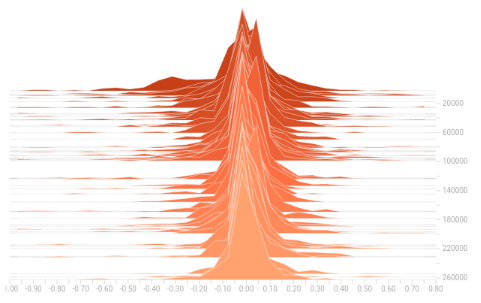
\includegraphics[scale=0.75]{cap5_train_histogram.png}
	\caption{Histograma temporal do erro classificação}
	\label{fig:cap5_train_histogram}
	Pode-se observar os erros se concentrando cada vez mais próximo de 0 a
	medida que o treinamento avança. A escala indicada são batches de 256
	imagens, portanto este gráfico o resultado após mais de 66 milhões de
	imagens (próprio autor).
\end{figure}

\begin{figure}[!htb]
	\centering
	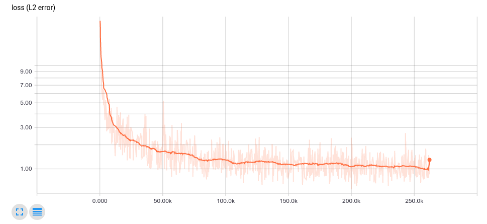
\includegraphics[scale=1]{cap5_erro_treinamento.png}
	\caption{Gráfico do erro de treinamento}
	\label{fig:cap5_erro_treinamento}
	Evolução da função de perda que o otimizador está minimizando, amortecido
	usando método média local. A abscissa é o número do batch, e cada batch
	possui 256 imagens (próprio autor).
\end{figure}

\subsection{Player}

\begin{figure}[!htb]
	\centering
	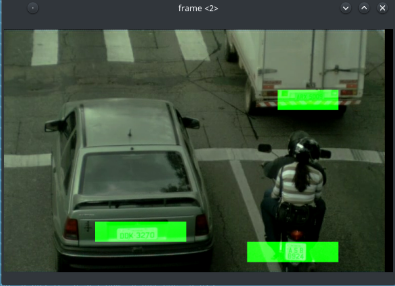
\includegraphics{cap5_tela_player.png}
	\caption{Interface com o usuário do módulo \emph{Player}}
	\label{fig:cap5_tela_player}
	No momento que a tela foi capturada o \emph{software} está exibindo um
	vídeo enquanto destaca as placas que está localizando (próprio autor).
\end{figure}

O quarto módulo de \emph{software} usa a rede neural treinada para reproduzir o
conteúdo de um vídeo ou da câmera enquanto destaca as placas de carros
localizadas. A figura \ref{fig:cap5_tela_player} mostra a interface do usuário
no momento em que está exibindo um vídeo quando três veículos estão passando.
As placas dos mesmos estão sendo destacadas.

O \emph{software} implementa o método de classificação proposto nesta
monografia por
completo. O método de binarização é um limiar simples em 0,75. Este valor
permite que quando a placa está transitando de uma partição para outra, ambas
as placas serão iluminadas momentaneamente antes da placa que ficou para trás
apagar.

Não foi implementado nenhum método para usar a correlação temporal das
informações coletadas.

Para o \emph{video1.avi} a rede neural é executada 288 vezes para frame do
vídeo, sendo que uma linha completa contendo 12 partições é fornecido para a
rede neural por vez.

O \emph{software} é capaz de operar em qualquer vídeo que possa ser lido pelo
\emph{OpenCV3} e pode usar a imagem da câmera do computador.

\section{Experimentos e Desempenho}

Nesta sessão serão apresentados os experimentos realizados com a implementação
do \emph{software} e os seus resultados.

\subsection{Desempenho de Localização}

Como o método de localização proposto é aproximado, a abordagem para teste de
desempenho é baseada na contagem de placas corretamente ou
incorretamente localizadas. Para que uma placa seja considerada corretamente
localizada basta que ela esteja a menos de 60 \emph{pixels} de distância na
largura e menos de 20 \emph{pixels} na altura. Estes limites foram escolhidos
por serem metade do tamanho das partições, que representa a distância na qual
a função que está sendo modelada pela rede neural deve ir à zero.
	
Para a medição de desempenho serão usadas as métricas \emph{precision}
(equação \ref{eq:precision}) e \emph{recall} (equação \ref{eq:recall}).

\noindent\begin{minipage}{.5\linewidth}
	\begin{equation} \label{eq:precision}
		\text{Precision} = \frac{vp}{vp + fp}
	\end{equation}
\end{minipage}
\begin{minipage}{.5\linewidth}
	\begin{equation} \label{eq:recall}
		\text{Recall} = \frac{vp}{vp + fn}
	\end{equation}
\end{minipage}

Onde $vp$ é o número de verdadeiros positivos, $fp$ é o número de falsos
positivos e $fn$ é o número de falsos negativos. Estes dados serão obtidos da
seguinte maneira:

\begin{itemize}

\item Quando o \emph{software} identificar uma placa em um ponto do \emph{frame} e
	houver uma placa entre as manualmente marcadas, tal que a distância entre
	os centros  das duas seja inferior ao erro, será contabilizado um
	\emph{verdadeiro positivo}, ou \emph{tp} (figura \ref{fig:cap5_tp-fn-fp},
	placa ``a'').
	A placa é removida da lista de placas manualmente marcadas para não
	ser usada novamente, pois já foi localizada (figura
	\ref{fig:cap5_tp-fn-fp}, placa ``b'').;

\item Se no caso anterior não houver placa manualmente marcada tal que o erro
	seja inferior ao máximo será contabilizado um falso positivo, ou \emph{fp}
	(figura \ref{fig:cap5_tp-fn-fp}, placa ``c'');

\item as placas que foram manualmente marcadas e não forem localizadas são
	contabilizadas como falso negativos, ou \emph{fn} (figura
	\ref{fig:cap5_tp-fn-fp}, placa ``A'').

\end{itemize}

\begin{figure}[!htb]
	\centering
	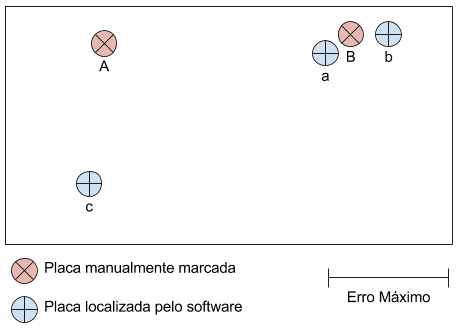
\includegraphics[scale=0.7]{cap5_tp-fn-fp.png}
	\caption{Contagem de acertos e erros de localização}
	\label{fig:cap5_tp-fn-fp}
	Cada círculo representa o centro de uma placa. Constam 1 \emph{verdadeiro
	positivo} (B/a), 2 falsos positivos (b, c), e um \emph{falso negativo} (A).
	Próximo a placa ``B'' foram localizadas duas placas, mas
	só há uma, então uma delas é contada como \emph{falso positivo}
	(próprio autor).
\end{figure}

Para usar usar corretamente o método proposto é preciso escolher um limiar de
classificação. Se o escore de uma partição for maior que este limiar
considera-se que a partição possui uma placa veicular. Como este escore afeta
as métricas \emph{precision} e \emph{recall}, foi feito um levantamento da
\emph{curva precision-recall} para determinar o valor mais apropriado de limiar
a ser usado. A tabela \ref{tbl:curva-pr} e o gráfico na figura
\ref{fig:cap5_res_curva-pr} esta curva para os dados de teste. Apenas para
referência, o gráfico também foi calculado para o set de treinamentos, por ser
maior, gerando o gráfico da figura \ref{fig:cap5_res_curva-pr-train}.

\noindent\begin{minipage}{.5\linewidth}
	\begin{equation} \label{eq:precision}
		\text{Precision} = \frac{vp}{vp + fp}
	\end{equation}
\end{minipage}
\begin{minipage}{.5\linewidth}
	\begin{equation} \label{eq:recall}
		\text{Recall} = \frac{vp}{vp + fn}
	\end{equation}
\end{minipage}

\begin{table}
	\center
	\caption{Erros e acertos de localização}
	\renewcommand{\arraystretch}{1.6}
	\begin{tabular}{ccc}
		\Xhline{6\arrayrulewidth}
		\textbf{Limiar} &
			\textbf{Recall} &
			\textbf{Precision} \\
		\Xhline{2\arrayrulewidth}
			0    & 100,0\%  &  3,44\% \\
			0,1  & 100,0\%  &  53,8\% \\
			0,14 & 100,0\%  &  57,9\% \\
			0,2  & 100,0\%  &  67,2\% \\
			0,3  & 100,0\%  &  78,0\% \\
			0,5  & 100,0\%  &  94.8\% \\
			0,7  & 100,0\%  &  94,8\% \\
			\textbf{0,8}  &  \textbf{96,7\%}  &  \textbf{98,9\%} \\
			0,9  &  94,6\%  &  98,9\% \\
			0,93 &  91,3\%  &  98,8\% \\
			0,97 &  80,4\%  &  98,7\% \\
			0,99 &  65,2\%  &  98,4\% \\
			1,01 &  19,6\%  & 100,0\% \\
		\Xhline{6\arrayrulewidth}
	\end{tabular}
	\label{tbl:curva-pr}
\end{table}

\begin{figure}[!htb]
	\centering
	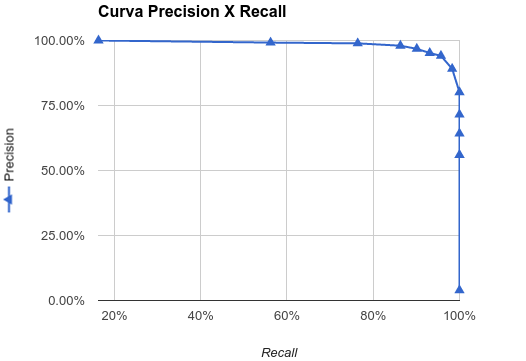
\includegraphics[scale=0.75]{cap5_res_curva-pr-train.png}
	\caption{Gráfico da curva Precision-Recall (amostras de treinamento)}
	\label{fig:cap5_res_curva-pr-train}
	Oserva-se uma curva semelhante a curva PR para o set de testes. Como este
	set é maior a forma é mais suave (próprio autor).
\end{figure}

\begin{figure}[!htb]
	\centering
	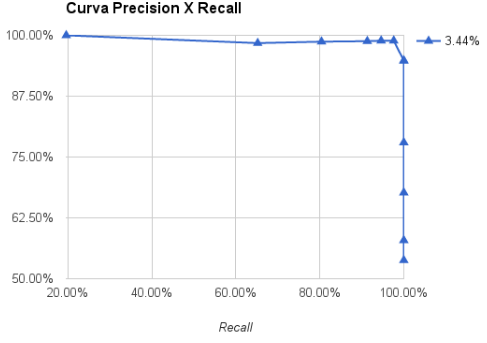
\includegraphics[scale=0.75]{cap5_res_curva-pr.png}
	\caption{Gráfico da curva Precision-Recall (amostras de teste)}
	\label{fig:cap5_res_curva-pr}
	Pode-se observar como o limiar de classificação afeta \emph{precision} e
	\emph{recall} (próprio autor).
\end{figure}

Tendo sido escolhido o limiar 0.8 para aceitar uma placa, as métricas
\emph{precision} e \emph{recall} foram calculados para todos os conjuntos
de dados marcados disponíveis, tanto de teste quanto de treinamento.
Os resultados obtidos estão apresentados na tabela
\ref{tbl:vp-fp-fn}. Os indicadores de desempenho foram melhores no
conjunto de dados de teste do que no conjunto de treinamento. Isso
se deve ao fato de que a implementação, como foi feita, não detecta
placas que estejam próximos a borda direita e
inferior da imagem. O set de testes foi preparado tomando cuidado para não usar
frames onde veículos se encontrem nesta região.

O resultado do \emph{precision}
no video2 foi apenas 59,0\%, causado pela quantidade excessiva de falso
positivos. Observou-se que uma única das sessões da imagem que pertence ao
asfalto, foi marcada em aproximadamente 50\% das frames como placa, gerando
falso positivos. Atribui-se este problema a resolução deste vídeo, que é $1080
\times 1920$, e portanto requer uma grande quantidade de marcações para que
seja coletada uma quantidade suficiente de amostras de ``não-placa'' para
eliminar este problema, já que o \emph{software} de coleta de exemplos de treinamento
tenta balancear a quantidade de exemplos positivos e negativos.


\begin{table}
	\center
	\caption{Erros e acertos de localização}
	\renewcommand{\arraystretch}{1.6}
	\begin{tabular}{p{4.5cm} c c c c c}
		\Xhline{6\arrayrulewidth}
		\textbf{Vídeo} &
			\textbf{VP} &
			\textbf{FP} &
			\textbf{FN} &
			\textbf{Precision} &
			\textbf{Recall} \\
		\Xhline{2\arrayrulewidth}
		\textbf{video1.avi (teste)} &
			\textbf{89} &
			\textbf{1} &
			\textbf{3} &
			\textbf{98,9\%} &
			\textbf{96,7\%} \\
		video1.avi (treinamento) & 217 & 11 & 16 & 95,2\% & 93,1\% \\
		video2.avi (treinamento) &  92 & 64 &  4 & 59,0\% & 95,8\% \\
		\Xhline{6\arrayrulewidth}
	\end{tabular}
	\label{tbl:vp-fp-fn}
\end{table}

\subsection{Função}

Como o método proposto envolve fazer a regressão de uma função, as primeiras
medições aqui apresentadas estão mostrando o resultado desse modelamento. As
figuras \ref{fig:cap5_res_func_1} e \ref{fig:cap5_res_func_2} mostram 3 carros,
uma moto e um ônibus, sendo que o classificador foi aplicado
\emph{pixel}-a-\emph{pixel} na
região próxima da placa, e o seu valor representado em um gráfico 3D. Este
gráfico pode ser comparado com o gráfico mostrado na figura
\ref{fig:func_a_modelar_3d}, que mostra o gráfico ideal.

Estes dados foram todos levantados usando o vídeo3.avi, que não usado para
treinamento. As cinco frames foram escolhidos ao acaso, garantindo-se apenas
que as cinco imagens sejam suficientemente diferentes umas das outras.

A capacidade de produzir estes gráficos foi incluído no \emph{software}
``\emph{player}'', e pode ser invocada para qualquer frame de qualquer vídeo.

\begin{figure}[!htb]
	\centering
	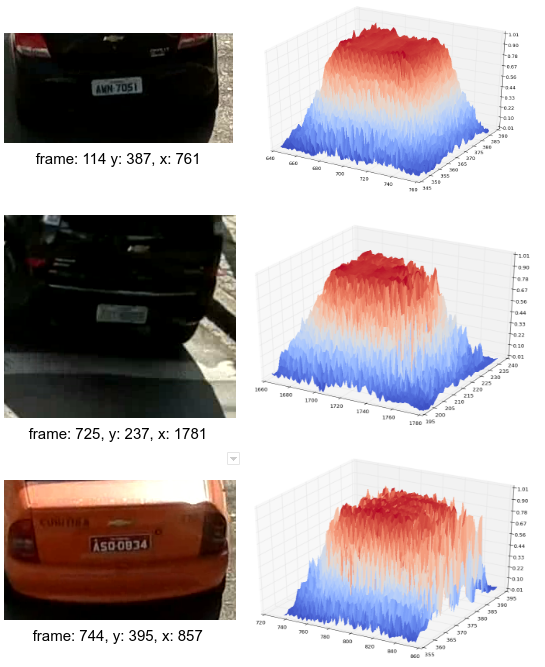
\includegraphics[scale=0.75]{cap5_res_func_1.png}
	\caption{Gráfico 3D da função aplicada a carros}
	\label{fig:cap5_res_func_1}
	São destacados três carros, um com boa textura, placa razoavelmente
	visível, outra com imagem com perda resultante de compactação, e um
	terceiro em posição, e cores diferentes, inclusive usando letras mais
	claras que o frame da placa. O gráfico mostra o resultado do classificador
	quando ele está centrada em cada um dos \emph{pixels} próximo à placa.
	As abiscissas referem-se as coordenadas do canto superior-esquerdo da
	partição, não ao seu centro (próprio autor).
\end{figure}

\begin{figure}[!htb]
	\centering
	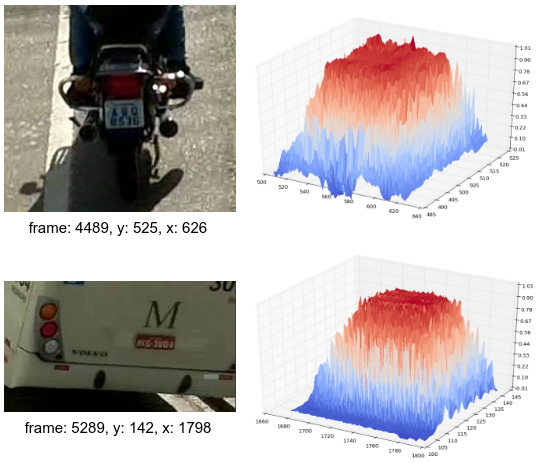
\includegraphics[scale=0.75]{cap5_res_func_2.png}
	\caption{Gráfico 3D da função aplicada a moto e ônibus}
	\label{fig:cap5_res_func_2}
	Observa-se uma moto e um veículo e o gráfico resultante de aplicar o
	classificador em torno das placas. As abiscissas referem-se as coordenadas
	do canto superior-esquerdo da partição, não ao seu centro (próprio autor).
\end{figure}

A figura \ref{fig:cap5_res_func_frame} mostra a rede neural sendo aplicada
na frame 11.197 do video1. Esta frame não faz parte do conjunto de treinamento.
Pode-se verificar claramente onde estão as duas placas veiculares.

\begin{figure}[!htb]
	\centering
	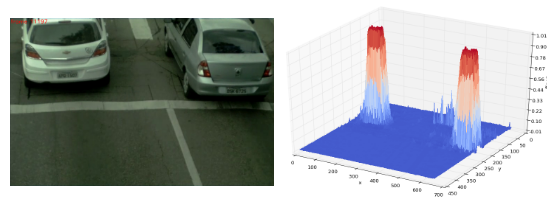
\includegraphics{cap5_res_func_frame.png}
	\caption{Gráfico 3D mostrando a função aplicada à uma frame inteira}
	\label{fig:cap5_res_func_frame}
	Pode-se ver claramente onde as placas dos dois veículos se encontram.
	(próprio autor).
\end{figure}

\subsection{Tempo de Classificação}
Para os testes de tempo de classificação foi usado o módulo \emph{player}. Este
módulo mostra uma janela com o vídeo sendo classificado enquanto envia para
\emph{stdout} uma série de informações de desempenho. Estes dados foram
usados nas medições relacionadas a tempo de classificação.


\begin{table}
	\center
	\caption{Taxa de Frames por Segundo}
	\renewcommand{\arraystretch}{1.6}
	\begin{tabular}{ccccc}
		\Xhline{6\arrayrulewidth}
		\textbf{Vídeo} &
			\textbf{Resolução} &
			\textbf{FPS (GPU)} &
			\textbf{FPS (CPU)} &
			\textbf{Melhoria} \\
		\Xhline{2\arrayrulewidth}
		camera     & $480  \times 640$  & 15,8 & 9.12 & 73\%  \\
		video1.avi & $480  \times 768$  & 14,8 & 8,08 & 84\%  \\
		video2.avi & $1080 \times 1920$ & 3,29 & 1,51 & 117\% \\
		video3.avi & $1080 \times 1920$ & 3,34 & 1,51 & 121\%  \\
		\Xhline{6\arrayrulewidth}
	\end{tabular}
	\label{tbl:player_fps}
\end{table}

Observa-se na tabela \ref{tbl:player_fps} que o \emph{player} não consegue
atingir a taxa de 25 frames por segundo
de nenhum dos três vídeos, mesmo com uso de GPU. A taxa de frames
aumenta consideravelmente quando a GPU é usada. Entre os casos
testados o ganho é maior quando a resolução do vídeo aumenta. A figura
\ref{fig:cap5_player_fps} mostra o resultado em forma de gráfico.

\begin{figure}[!htb]
	\centering
	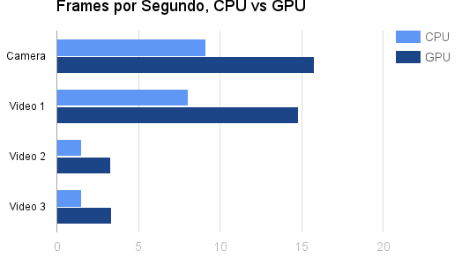
\includegraphics{cap5_player_fps.png}
	\caption{Taxa de frames por segundo no módulo \emph{Player}}
	\label{fig:cap5_player_fps}
	Gráfico mostrando desempenho em frames por segundo para localizar placas na
	câmera VGA do computador, e nos três vídeos. Computador é um Core i5 com
	placa de vídeo GTX 750M. Maior é melhor (próprio
	autor).
\end{figure}

O \emph{player} envia para o \emph{stdout} o tempo gasto em cada uma das
tarefas durante o processamento da frame. Coletando-se estes dados e
calculando-se as médias do tempo gasto em cada tarefa foi gerado o
gráfico na figura \ref{fig:cap5_frame_benchmark}.

\begin{figure}[!htb]
	\centering
	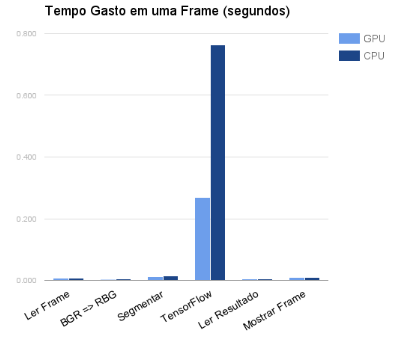
\includegraphics{cap5_frame_benchmark.png}
	\caption{Tempo gasto em cada subtarefa no processamento de uma
		\emph{frame}}
	\label{fig:cap5_frame_benchmark}
	Gráfico mostra que, ao processar um vídeo $1080 \times 1920$ a grande
	maioria do tempo é gasto executando o grafo do \emph{TensorFlow}. Outras
	tarefas executadas pelo código em Python consomem um percentual
	pequeno do tempo da frame. Computador é um Core i5 com
	placa de vídeo GTX 750M (próprio autor).
\end{figure}

Pode-se ver claramente que a vasta maioria do tempo é gasta executando os
grafos do \emph{TensorFlow}. Também foi possível confirmar que o ganho do
desempenho no caso do uso do GPU foi consequência do \emph{TensorFlow}
consumir menos tempo para executar. Observou-se que na implementação CPU
o \emph{TensorFlow} tomou 94,9\% do tempo de processamento da frame, e no
caso que usa GPU tomou 88,1\%.
